% ---------------------------------------------------------------------------
% Author guideline and sample document for EG publication using LaTeX2e input
% D.Fellner, v1.13, Nov 13, 2007

\documentclass{egpubl}

% --- for  Annual CONFERENCE
% \ConferenceSubmission % uncomment for Conference submission
% \ConferencePaper      % uncomment for (final) Conference Paper
% \STAR                 % uncomment for STAR contribution
% \Tutorial             % uncomment for Tutorial contribution
% \ShortPresentation    % uncomment for (final) Short Conference Presentation
%
% --- for  CGF Journal
% \JournalSubmission    % uncomment for submission to Computer Graphics Forum
% \JournalPaper         % uncomment for final version of Journal Paper
%
% --- for  CGF Journal: special issue
% \SpecialIssueSubmission    % uncomment for submission to Computer Graphics Forum, special issue
% \SpecialIssuePaper         % uncomment for final version of Journal Paper, special issue
%
% --- for  EG Workshop Proceedings
% \WsSubmission    % uncomment for submission to EG Workshop
% \WsPaper         % uncomment for final version of EG Workshop contribution
%

\electronicVersion % can be used both for the printed and electronic version

% !! *please* don't change anything above
% !! unless you REALLY know what you are doing
% ------------------------------------------------------------------------

% for including postscript figures
% mind: package option 'draft' will replace PS figure by a filname within a frame
\ifpdf \usepackage[pdftex]{graphicx} \pdfcompresslevel=9
\else \usepackage[dvips]{graphicx} \fi

\PrintedOrElectronic

% prepare for electronic version of your document
\usepackage{t1enc,dfadobe}

\usepackage[utf8]{inputenc}
\usepackage{egweblnk}
\usepackage{cite}
\usepackage{comment}
\usepackage{amssymb}
\usepackage{amsmath}
\usepackage{tikz}
\usetikzlibrary{arrows,chains,matrix,positioning,scopes}

% For backwards compatibility to old LaTeX type font selection.
% Uncomment if your document adheres to LaTeX2e recommendations.
\let\rm=\rmfamily    \let\sf=\sffamily    \let\tt=\ttfamily
\let\it=\itshape     \let\sl=\slshape     \let\sc=\scshape
\let\bf=\bfseries

% end of prologue

\newcommand{\bigO}{\mathcal{O}}
\newcommand{\ambush}{A*mbush}
\newcommand{\astar}{A*}
\newcommand{\pambush}{P-A*mbush}
\newcommand{\rambush}{R-A*mbush}
\newcommand{\sarambush}{SAR-A*mbush}

\title[Ambush]%
      {Pruebas de Generaci\'on de Emboscadas Utilizando A*mbush}

% for anonymous conference submission please enter your SUBMISSION ID
% instead of the author's name (and leave the affiliation blank) !!
\author[K. Fernandes \& C. Chang]
       {K. Fernandes$^{1,2}$
        y C. Chang$^{1}$
        \\
         $^1$Departamento de Computaci\'on y Tecnolog\'ia de la
         Informaci\'on, Universidad Sim\'on Bol\'ivar, Venezuela\\
         $^2$INESC TEC, Porto, Portugal
      }

\begin{document}
\noEGpagenumber

\maketitle

\begin{abstract}
La secci\'on de RESUMEN debe tener el resumen del trabajo en idioma
español e ingl\'es. El resumen en español debe preceder al resumen
en ingl\'es y debe llevar por t\'itulo la palabra RESUMEN. Ambas
versiones del resumen deben tener alineaci\'on justificada, en
formato de una columna, y deben estar ubicadas debajo de la
afiliaci\'on del  autor. El titulo del resumen debe usar una fuente
Times tamaño 9, debe estar en negritas, debe estar alienado a la
izquierda  y debe estar escrito en may\'usculas. La secci\'on de
resumen completa, incluyendo ambas versiones y los keywords, no
debe exceder las 3.5 pulgadas (8.89 cm) de largo.
\\
\\
\textnormal{\textbf{ABSTRACT}}
\\
\\
The ABSTRACT is to be in fully-justified italicized text, between
two horizontal lines, in one-column format, below the author and
affiliation information. Use the word "Abstract" as the title, in
9-point Times, boldface type, left aligned to the text, fully
capitalized. The abstract is to be in 9-point, single-spaced type.

%
\begin{keywords}
A*, estrategias grupales, b\'usqueda de caminos, grafos.
\end{keywords}

\end{abstract}
\section{Introducci\'on}

En el \'area de Inteligencia Artificial para Videojuegos, la generaci\'on
de conductas inteligentes ha sido un reto constante \cite{MF09}, frecuentemente
derivado en el desarrollo de acciones prestablecidas que el usuario puede
f\'acilmente identificar despu\'es de varias ejecuciones del juego.
Esta caracter\'istica es a\'un m\'as com\'un cuando se trata de la generaci\'on
de movimientos t\'acticos y estrat\'egicos grupales, los cuales suelen ser sumamente
complejos de implementar.

Un problema muy tratado en la literatura es la b\'usqueda de caminos
a un punto com\'un, por parte de grupos de agentes dentro de un juego
\cite{MF09}. Este punto suele venir dado por un lugar en el mapa de juego,
potencialmente la posici\'on del oponente. El esquema regularmente utilizado
es generar caminos de costo m\'inimo \cite{HNR72} \cite{RN93}
hacia este punto, sobre el grafo inducido por el mapa del juego. Es
muy probable, que estos caminos confluyan, evitando la diversidad de
rutas y exploraci\'on del mapa.

Al efectuar una persecuci\'on al oponente, la utilizaci\'on de caminos
\'optimos como estrategia deja muchos espacios de escapatoria libres,
por lo que es de especial inter\'es generar mecanismos de diversificaci\'on de
rutas que generen situaciones de emboscada.

\textbf{
En este punto hablar de nuestra soluci\'on y de como esta prob\'o ser
correcta. Mencionar que este art\'iculo pretende ser un soporte adicional
a los dos anteriores para demostrar la validez de las distintas variantes
de forma exhaustiva as\'i como tambi\'en de presentar una nueva m\'etrica
que permite medir de forma m\'as refinada el grado de emboscada.
}

\begin{comment}
La t\'ecnica expuesta pr\'oximamente es adaptable a muchos contextos en
los que, si bien no es necesaria una situaci\'on de emboscada, es
importante generar diversidad de caminos con el fin de no sobresaturar
ciertos sectores del grafo subyacente. Ejemplo de estos son controladores
de tr\'afico, enrutamiento de paquetes f\'isicos o digitales \cite{TMSV03},
rob\'otica, entre otros.
\end{comment}
\section{Trabajos Relacionados}
\label{sec:state_of_the_art}

Este trabajo se centra en el estudio del m\'etodo expuesto
previamente por Fern\'andez y colaboradores \cite{FGC12e}\cite{FGC12}.
Enfoques alternativos a \'este fueron propuestos por Silver \cite{Sil06}
y por van Toll y colaboradores \cite{TCG12}.

En el trabajo propuesto por Silver \cite{Sil06}, denominado
\textit{Space-Time \astar}, se plantea una variante de $A^*$ 
donde se tiene un grafo no dirigido en forma de cuadrícula,
con función de costos común para todos los agentes y 
constante entre cada par de nodos.
El objetivo principal de dicho trabajo es evitar el paso de
dos agentes por un mismo nodo en un instante de tiempo dado.
La variación planteada incluye una extensión en el número
de dimensiones de \astar. Se considera, además de la posición
de los agentes, el tiempo transcurrido. Dicha variación tiene
un costo añadido en tiempo y memoria considerable debido a que
se incrementa el tamaño del espacio de búsqueda. Aunque el objetivo
final de las soluci\'on es diferente, la estudiada en el actual
trabajo presenta una clara ventaja sobre \textit{Space-Time A$^*$}
en varios aspectos. En primer lugar, resuelve con un algoritmo
de menor complejidad de c\'omputo problemas m\'as generales, debido a
que permite la utilizaci\'on de grafos dirigidos con costos de arcos
variables. Asimismo, se puede trabajar con agentes que
tengan grafos distintos entre sí.
Por otro lado, en el caso de tener agentes con distintas velocidades,
\textit{Space-Time A$^*$} genera un espacio de búsqueda en extremo
denso, cuando la velocidad relativa entre los e\-le\-men\-tos del juego es
alta. En cambio, $A^*mbush$ no se ve afectado por la diferencia de 
velocidades entre los agentes.
Asignando costos homogéneos para cada arco e incremento infinito
sobre nodos o arcos ocupados, el problema que resuelve $A^*mbush$
se reduce al problema planteado para \textit{Space-Time
A$^*$}.

El segundo trabajo mencionado, desarrollado por van Toll y otros
\cite{TCG12}, muestra un enfoque basado en densidades para generar
diversidad de caminos. Sin embargo, la diversificaci\'on de caminos
es dada s\'olo al alcanzar un gran n\'umero de agentes atravesando una
misma \'area, por lo que se torna infactible en los casos estudiados
en este trabajo, donde se pretende alcanzar emboscadas utilizando
el m\'inimo n\'umero de agentes posible.

\begin{minipage}{0.3\textwidth}

\section*{Formal Problem Definition}
\begin{itemize}
\item Let $G = (V,E)$ be a \textbf{graph} (directed or undirected).

\item Let $A$ be a \textbf{set of agents} that want to reach a point
$t \in V$. Every agent $i \in A$, is located in a node of the
graph. Let $pos(i)$ be the position of the agent $i$.

\item A function over $i$ is defined for  determining the
\textbf{cost} of the displacement of the agents  through the graph
$\lambda_i : E \longrightarrow \mathbb{R}^{\geq 0}$.

\item Let $path(i)$ having $i \in A$, be the \textbf{path} that the 
agent $i$ is taking to reach node $t$.

\item The \textbf{degree of ambush} towards the node $t$ is defined as:\\

$\Phi(t) = \dfrac{|\{ i : path(j) = <pos(j),\ \ldots,\ i,\ t>, j \in A\}|}
{\min(|\{ <i,t> : <i,t> \in E \} |,|A|) }$

\end{itemize}
\end{minipage}
\begin{minipage}{0.3\textwidth}
\section*{A*mbush}

\begin{itemize}

\item A$^*$mbush is an $A^*$-based algorithm that solves the
ambush generation problem. 

\item It consists of a \textbf{modification} of the $g$ function,
that favours path diversity. We will call this function $g'$.

\item Let $\Psi(v,i) = 1+(\# j : j \in A \wedge v \in path(j))$,
be the number of agents different from agent $i$, that have the 
node $v$ in their paths towards $t$ plus one.

\item $g'(pos(i),i) = 0$ for the initial node.

\item $g'(w, i) = g'(v,i) + \lambda_i(<v,w>) \cdot \Psi(w,i)^2$
for every expanded edge $<v,w>$.

\item The properties of $A^*$ are preserved. Nevertheless, the path
\textbf{might not be optimal} for the original costs function $g$.

\end{itemize}

\end{minipage}
\section{Experimentos}
\label{sec:experiments}

Para cada experimento se estudian cinco algoritmos:
una implementaci\'on base de \astar que sirve de referencia,
una implementaci\'on de caminos simples aleatorios mediante
b\'usqueda en profundidad, \ambush, \pambush con mecanismo
de prioridad determinado por la distancia real de los agentes
a la meta y finalmente, \sarambush.

presentan resultados del incremento medio porcentual de los caminos.
Para cada topolog\'ia de grafo, se generan aleatoriamente 100 grafos,
sobre los cuales se ejecutan experimentos con 100 disposiciones distintas
de agentes y del nodo objetivo.
Para cada uno de estos algoritmos se muestra el valor de emboscada
utilizando la m\'etrica originalmente propuesta y utilizando la
m\'etrica propuesta en el presente trabajo. El n\'umero de agentes
es variado con el fin de mostrar su impacto en el grado de emboscada
y en el incremento derivado de la escogencia de caminos sub\'optimos.
Adem\'as se muestran resultados con las dos instancias de mapas ($g1$ y $g2$)
presentadas en el trabajo previo \cite{FGC12} con 60 y 85 nodos
respectivamente. Estos mapas provienen de la poligonalizaci\'on del mapa
de juego en pol\'igonos. Estas restricciones son ampliamente utilizadas
en juegos\cite{MF09}. Estos grafos se pueden visualizar en la figura \ref{fig:gs}.

\begin{figure}[htb]
	\begin{center}
		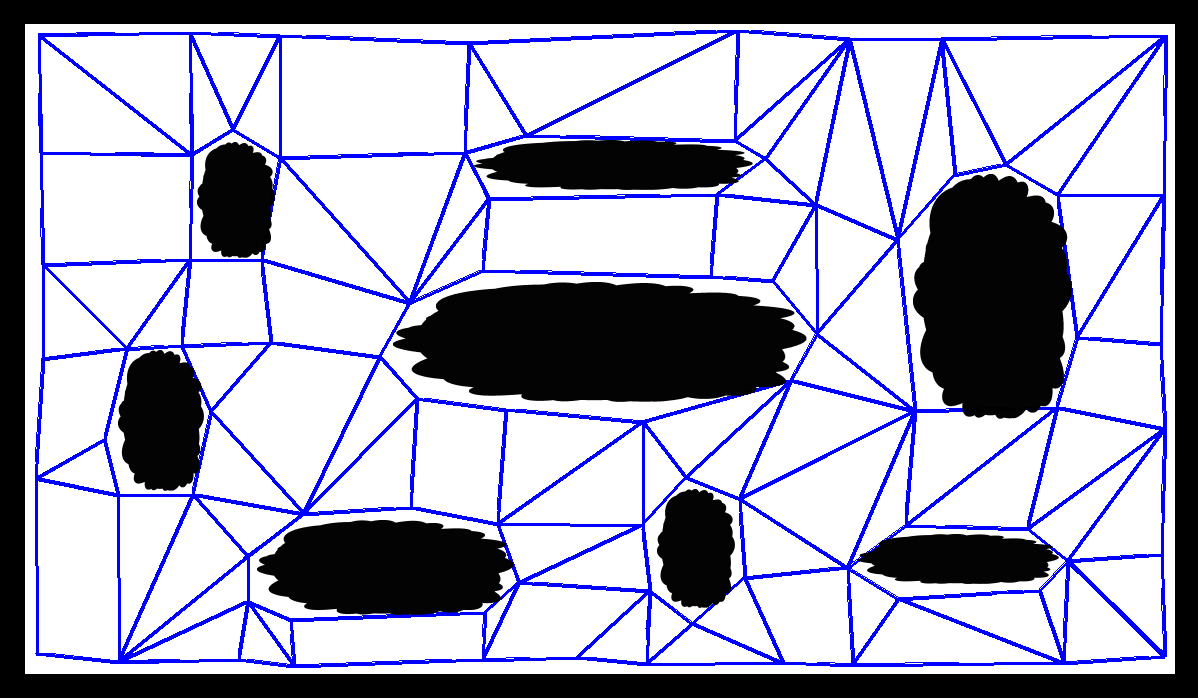
\includegraphics[scale=0.23]{figures/g1.png}
		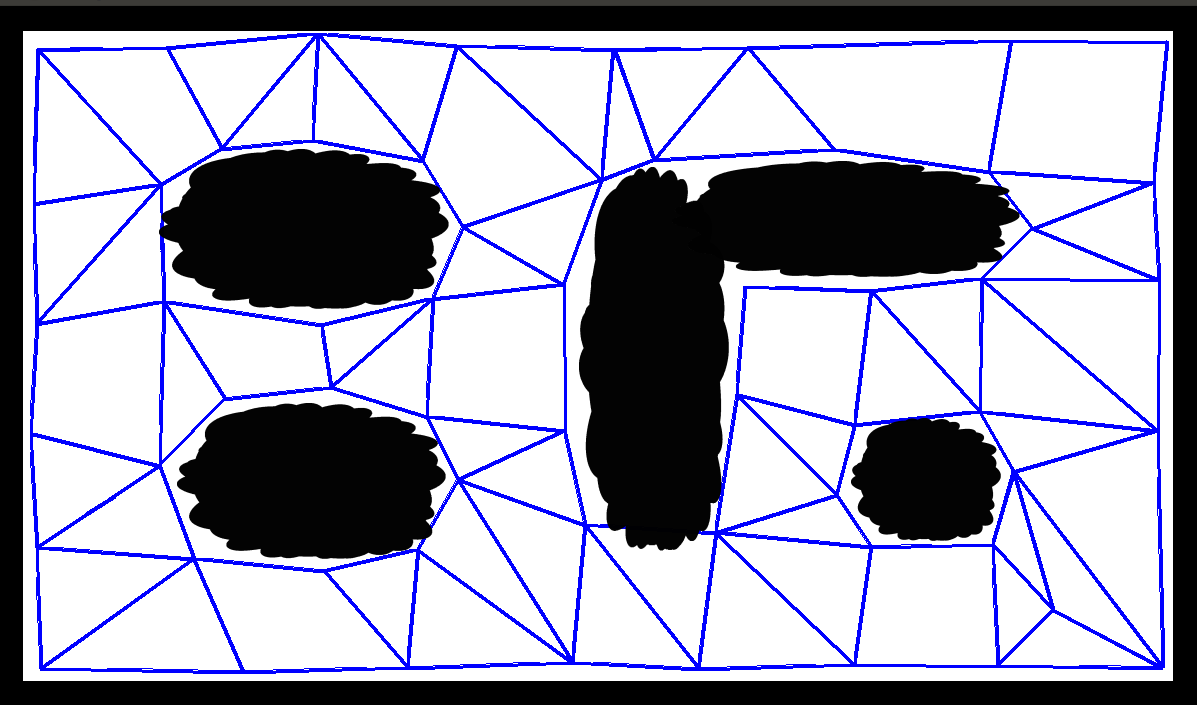
\includegraphics[scale=0.23]{figures/g2.png}
	\end{center}
	\caption{\label{fig:gs}
	     \textbf{Arriba:} Mapa 1 poligonalizado (60 pol\'igonos).
	     \textbf{Abajo:} Mapa 2 poligonalizado (85 pol\'igonos).
     }
\end{figure}

\section{Conclusiones y Trabajo Futuro}
\label{sec:conclusions}

\ambush\ y sus variantes muestran una evidente mejora en la conducta de
emboscada, con un c\'omputo adicional poco significativo con respecto
al algoritmo base de generaci\'on de caminos m\'inimos \astar.

Como se pudo apreciar en la secci\'on \ref{sec:experiments}, ninguna
de las variantes de \ambush\ muestra resultados inferiores a los obtenidos
por \astar. Adem\'as, todas las variaciones mostraron no ser gravemente
afectadas por diferencias significativas en el tamaño de los grafos y
del n\'umero de agentes. Dada la diversidad de situaciones planteadas
en los experimentos, se puede afirmar que \ambush\ muestra un comportamiento
estable y efectivo. El tipo de grafos bajo los cuales \ambush\ y sus
variantes presentaron menor eficacia fueron en los grafos con modelo
Dorogovtsev-Mendes, en los cuales, si bien el algoritmo fue capaz de
incrementar significativamente el grado de emboscada, no alcanz\'o
los resultados obtenidos con los otros tipos de grafo.

\ambush\ genera comportamientos de emboscada inteligentes para situaciones
en las que múltiples agentes necesitan alcanzar un objetivo común. En
contraste con estrategias preestablecidas, regularmente implementadas para
situaciones específicas de cada juego, que derivan en situaciones repetitivas,
\ambush\ logra fomentar situaciones va\-ria\-das de emboscada dentro del 
comportamiento táctico grupal de los agentes.

En este trabajo se present\'o una nueva m\'etrica para medir el grado de
emboscada que, al utilizar una mayor cantidad de informaci\'on es capaz
de identificar aquellos casos en los cuales las salidas dejadas al
adversario son de hecho imposible de cubrir por alguno de los agentes.
La m\'etrica propuesta eval\'ua de forma m\'as estable la calidad de
emboscada independientemente de la topolog\'ia del grafo base.
La métrica propuesta en el presente trabajo es mejor que la anterior
para medir el nivel de emboscada, como se refleja en la mayoría de
los experimentos.

En el futuro, se pretende extender este trabajo incluyendo informaci\'on
de capacidad para cada nodo, de tal forma de incluir restricciones
f\'isicas del mundo en el c\'alculo de la ruta. Adem\'as, se pretende
incluir restricciones en la comunicaci\'on que los agentes son capaces
de establecer entre si, para de esta forma poder adaptarse a situaciones
en las cuales existe s\'olo observailidad parcial entre los agentes.

%\begin{comment}

\section{Introduction}

Please follow the steps outlined in this document very carefully when
submitting your manuscript to Eurographics.

You may as well use the \LaTeX\ source as a template to typeset your own
paper. In this case we encourage you to also read the \LaTeX\ comments
embedded in the document.

%-------------------------------------------------------------------------
\section{Instructions}

Please read the following carefully.

%-------------------------------------------------------------------------
\subsection{Language}

All manuscripts must be in English.

%-------------------------------------------------------------------------
\subsection{Margins and page numbering}

All printed material, including text, illustrations, and charts,
must be kept within a print area 6.31 inches (16.03 cm) wide by
9.10 inches (23.13 cm) high. Do not write or print anything
outside the print area. Number your pages on odd sites right
above, on even sites left above, no page number on the first site.
Do not use page numbering within the final version of your paper.


%------------------------------------------------------------------------
\subsection{Formatting your paper}

All text with the exception of the abstract must be in a two-column format.
The total allowable width of the text area -- including header and footer
lines -- is 161\,mm (6.34 inch) wide by 231\,mm (9.10 inch) high.

Columns are to be 76\,mm (3.0 inch) wide, with a 8\,mm (0.315 inch) space
between them.

The space between the header line and the first line of the text body and
between the last line of the text body and the footer line is 5\,mm
(0.196 inch) each.

%-------------------------------------------------------------------------
\subsection{Type-style and fonts}

Wherever Times is specified, Times Roman may also be used. If
neither is available on your word processor, please use the font
closest in appearance to Times that you have access to. Only
Type-1 fonts will be accepted.

MAIN TITLE. The title should be in Times 17-point, boldface type and
centered. Capitalize the first letter of nouns, pronouns, verbs, adjectives,
and adverbs; do not capitalize articles, coordinate conjunctions, or
prepositions (unless the title begins with such a word). Leave two blank
lines after the title.

AUTHOR NAME(s) and AFFILIATION(s) are to be centered beneath the title and
printed in Times 9-point, non-boldface type. This information is to be
followed by two blank lines.

The ABSTRACT is to be in a one-column format. The MAIN TEXT is to be in a
two-column format.

MAIN TEXT. Type main text in 9-point Times, single-spaced. Do \emph{not} use
double-spacing. All paragraphs should be indented 1 em (the length of the
dash in the actual font). Make sure your text is fully justified -- that is,
flush left and flush right. Please do not place any additional blank lines
between paragraphs. Figure and table captions should be 9-point Times
boldface type as in Figure~\ref{fig:firstExample}.

\noindent Long captions should be set as in Figure~\ref{fig:ex1} or
Figure~\ref{fig:ex3}.

\begin{figure}[htb]
   % an empty figure just consisting of the caption lines
   \caption{\label{fig:ex1}
     'Empty' figure only to serve as an example of long caption requiring
     more than one line. It is not typed centered but aligned on both sides.}
\end{figure}

\noindent
Figures which need the full textwidth can be typeset as Figure~\ref{fig:ex3}.

\noindent Callouts should be 9-point Times, non-boldface type. Initially
capitalize only the first word of section titles and first-, second-, and
third-order headings.

FIRST-ORDER HEADINGS. (For example, \textbf{1. Introduction}) should be Times
9-point boldface, initially capitalized, flush left, with one blank line
before, and one blank line after.

SECOND-ORDER HEADINGS. (For example, \textbf{2.1. Language}) should be Times
9-point boldface, initially capitalized, flush left, with one blank line
before, and one after. If you require a third-order heading (we discourage
it), use 9-point Times, boldface, initially capitalized, flush left, preceded
by one blank line, followed by a period and your text on the same line.

The headline \emph{(authors / title)} must be shortened if it uses the full
two column width of the main text.
There must be enough space for the page numbers. Please use ``et al.'' if
there are more than three authors and specify a shortened version for your title.
%-------------------------------------------------------------------------
\subsection{Footnotes}

Please do \emph{not} use footnotes at all!


%-------------------------------------------------------------------------
\subsection{References}

List all bibliographical references in 9-point Times, single-spaced, at the
end of your paper in alphabetical order. When referenced in the text, enclose
the citation index in square brackets, for example~\cite{Lous90}. Where
appropriate, include the name(s) of editors of referenced books.

For your references please use the following algorithm:
\begin{itemize}
\item \textbf{one} author: first 3 chars plus year --
      e.g.\ \cite{Lous90}
\item \textbf{two}, \textbf{three} or \textbf{four} authors: first char
      of each family name plus year --  e.g.\ \cite{Fellner-Helmberg93}
      or \cite{Kobbelt97-USHDR} or \cite{Lafortune97-NARF}
\item \textbf{more than 4} authors: first char of family name from
      first 3 authors followed by a '*' followed by the year --
      e.g.\ \cite{Buhmann:1998:DCQ} or \cite{FolDamFeiHug.etal93}
\end{itemize}

For BibTeX users a style file \ \texttt{eg-alpha.bst} \ is available which
uses the above algorithm.

%-------------------------------------------------------------------------
\subsection{Illustrations, graphs, and photographs}

All graphics should be centered.

%%%
%%% Figure 1
%%%
\begin{figure}[htb]
  \centering
  % the following command controls the width of the embedded PS file
  % (relative to the width of the current column)
  \includegraphics[width=.8\linewidth]{sampleFig}
  % replacing the above command with the one below will explicitly set
  % the bounding box of the PS figure to the rectangle (xl,yl),(xh,yh).
  % It will also prevent LaTeX from reading the PS file to determine
  % the bounding box (i.e., it will speed up the compilation process)
  % \includegraphics[width=.95\linewidth, bb=39 696 126 756]{sampleFig}
  %
  \parbox[t]{.9\columnwidth}{\relax
           For all figures please keep in mind that you \textbf{must not}
           use images with transparent background!
           }
  %
  \caption{\label{fig:firstExample}
           Here is a sample figure.}
\end{figure}

If your paper includes images, it is very important that they are of
sufficient resolution to be faithfully reproduced.

To determine the optimum size (width and height) of an image, measure
the image's size as it appears in your document (in millimeters), and
then multiply those two values by 12. The resulting values are the
optimum $x$ and $y$ resolution, in pixels, of the image. Image quality
will suffer if these guidelines are not followed.

Example 1:
%
An image measures 50\,mm by 75\,mm when placed in a document. This
image should have a resolution of no less than 600 pixels by 900
pixels in order to be reproduced faithfully.

Example 2:
%
Capturing a screenshot of your entire $1024 \times 768$ pixel display
monitor may be useful in illustrating a concept from your research. In
order to be reproduced faithfully, that $1024 \times 768$ image should
be no larger than 85 mm by 64 mm (approximately) when placed in your
document.


%-------------------------------------------------------------------------
\subsection{Color}

\textbf{Please observe:} as of 2003 publications in the proceedings of the
Eurographics Conference can use color images throughout the paper. No
separate color tables are necessary.

However, workshop proceedings might have different agreements!
Figure~\ref{fig:ex3} is an example for creating color plates.

%------------------------------------------------------------------------
\subsection{Embedding of Hyperlinks / Typesetting of URLs}

Due to the use of the package \texttt{hyperref} the original behavior
of the command $\backslash$\texttt{url} from the package \texttt{url}
is not available. To circumvent this problem we either recommend to
use the command $\backslash$\texttt{httpAddr} from the
included package \texttt{egweblnk} (see below) or to replace the
command $\backslash$\texttt{url} by the command $\backslash$\texttt{webLink}
-- e.g. in cases where $\backslash$\texttt{url} has been used
widely in BibTeX-References. In the latter case we suggest to run
BibTeX as usual and then replace all occurences of $\backslash$\texttt{url}  by
$\backslash$\texttt{webLink}

\noindent
The provided commands for hyperlinks, in a nutshell, are:

\begin{description} \itemsep 1ex
\item [\webLinkFont $\backslash$httpAddr \{URL without leading 'http:'\}]
      \mbox{}\\
      e.g. \  \httpAddr{//diglib.eg.org/EG/DL/WS}

\item[\webLinkFont $\backslash$ftpAddr \{URL without leading 'ftp:'\}]
      \mbox{}\\
      e.g. \  \ftpAddr{//www.eg.org/EG/DL/ftpupload}

\item[\webLinkFont $\backslash$URL \{url\}]
      \mbox{}\\
      e.g. \  \URL{http://www.eg.org/EG/DL/WS}

\item[\webLinkFont $\backslash$MailTo \{Email addr\}]
      \mbox{}\\
      e.g. \  \MailTo{publishing@eg.org}

\item[\webLinkFont $\backslash$MailToNA \{emailName\}\{@emailSiteAddress\}]
      \mbox{}\\
      e.g. \  \MailToNA{publishing}{@eg.org}

\item[\webLinkFont $\backslash$webLink\{URL without hyperlink creation\}]
      \mbox{}\\
      e.g. \  \webLink{http://www.eg.org/some_arbitrary_long/but_useless/URL}

\end{description}


%------------------------------------------------------------------------
\subsection{PDF Generation}

Your final paper should be delivered as a PDF document with all typefaces
embedded. \LaTeX{} users should use \texttt{dvips} and \texttt{ps2pdf} to
create this PDF document. Adobe Acrobat Distiller may be used in place of
\texttt{ps2pdf}.

Adobe PDFWriter is \emph{not} acceptable for use. Documents created with
PDFWriter will be returned to the author for revision. \texttt{pdftex} and
\texttt{pdflatex} (and its variants) can be used only if the author can
make certain that all typefaces are embedded and images are not downsampled
or subsampled during the PDF creation process.

Users with no access to these PDF creation tools should make available a
PostScript file and we will make a PDF document from it.


The PDF file \emph{must not} be change protected.

%------------------------------------------------------------------------
\subsubsection*{Configuration Notes: dvips / ps2pdf / etc.}

\noindent
\texttt{dvips} should be invoked with the \texttt{-Ppdf} and \texttt{-G0}
flags in order to use Type 1 PostScript typefaces:

\begin{verbatim}
    dvips -t a4 -Ppdf -G0 -o my.ps my.dvi
\end{verbatim}


\noindent
If you are using version 7.x of GhostScript, please use the following method of invoking \texttt{ps2pdf}, in
order to embed all typefaces and ensure that images are not downsampled or subsampled in the PDF
creation process:

\begin{verbatim}
  ps2pdf -dMaxSubsetPct=100 \
         -dCompatibilityLevel=1.3 \
         -dSubsetFonts=true \
         -dEmbedAllFonts=true \
         -dAutoFilterColorImages=false \
         -dAutoFilterGrayImages=false \
         -dColorImageFilter=/FlateEncode \
         -dGrayImageFilter=/FlateEncode \
         -dMonoImageFilter=/FlateEncode \
         mypaper.ps mypaper.pdf
\end{verbatim}


If you are using version 8.x of GhostScript, please use this method in place of the example above:
\begin{verbatim}
  ps2pdf -dPDFSETTINGS=/prepress \
         -dCompatibilityLevel=1.3 \
         -dAutoFilterColorImages=false \
         -dAutoFilterGrayImages=false \
         -dColorImageFilter=/FlateEncode \
         -dGrayImageFilter=/FlateEncode \
         -dMonoImageFilter=/FlateEncode \
         -dDownsampleColorImages=false \
         -dDownsampleGrayImages=false \
         mypaper.ps mypaper.pdf
\end{verbatim}

%------------------------------------------------------------------------
\subsubsection*{Configuration Notes: pdftex / pdflatex / etc.}

\noindent
Configuration of these tools to embed all typefaces can be accomplished by editing the \texttt{updmap.cfg} file
to enable inclusion of the standard (or base) 14 typefaces.

Linux users can run the \texttt{updmap} script to do this:
\begin{verbatim}
updmap --setoption pdftexDownloadBase14 true
\end{verbatim}

Windows users should edit the \texttt{updmap.cfg} files found in their TeX installation directories (one or both
of the following may be present):
\begin{verbatim}
  INSTALLDIR\texmf\web2c\updmap.cfg
  INSTALLDIR\localtexmf\miktex\config\updmap.cfg
\end{verbatim}

Ensure the value for \texttt{pdftexDownloadBase14} is "true," and then follow the instructions found here:
\httpAddr{//docs.miktex.org/manual/} to update your MikTeX installation.

%------------------------------------------------------------------------
\subsubsection*{Configuration Notes: Acrobat Distiller}

We recommend to download and install the version of the ``CMW'' Adobe Acrobat Distiller job options file
appropriate for your operating system and version of Acrobat from the following URL:

\httpAddr{//www.cadmusmediaworks.com/index2.html}\\
in the ``(Operating System)/Applications/Distiller Settings'' folder. The ``CMW'' job options file embeds
all typefaces and does not downsample or subsample images when creating the PDF document.
%------------------------------------------------------------------------
\subsection{Copyright forms}

You must include your signed Eurographics copyright release form
when you submit your finished paper. We MUST have this form before
your paper can be published in the proceedings.

%-------------------------------------------------------------------------
\subsection{Conclusions}

Please direct any questions to the production editor in charge of
these proceedings.

%-------------------------------------------------------------------------

%-------------------------------------------------------------------------
\newpage


\begin{figure*}[tcb]
  \centering
  \mbox{} \hfill
  % the following command controls the width of the embedded PS file
  % (relative to the width of the current column)
  \includegraphics[width=.3\linewidth]{sampleFig}
  % replacing the above command with the one below will explicitly set
  % the bounding box of the PS figure to the rectangle (xl,yl),(xh,yh).
  % It will also prevent LaTeX from reading the PS file to determine
  % the bounding box (i.e., it will speed up the compilation process)
  % \includegraphics[width=.3\linewidth, bb=39 696 126 756]{sampleFig}
  \hfill
  \includegraphics[width=.3\linewidth]{sampleFig}
  \hfill \mbox{}
  \caption{\label{fig:ex3}%
           For publications with color tables (i.e., publications not offering
           color throughout the paper) please \textbf{observe}:
           for the printed version -- and ONLY for the printed
           version -- color figures have to be placed in the last page.
           \newline
           For the electronic version, which will be converted to PDF before
           making it available electronically, the color images should be
           embedded within the document. Optionally, other multimedia
           material may be attached to the electronic version. }
\end{figure*}

\end{comment}


\bibliographystyle{eg-alpha}
\bibliography{egbibsample}

\end{document}
